\chapter{Воздушные суда от мала до велика}%
\label{ch:aircraft-chapter}

Глава посвящена исследованию различных свойств воздушных судов 
на основе базы знаний международного проекта Викиданные. 
В ходе исследования с помощью SPARQL-запросов, вычисляемых на объектах типа <<Воздушные суда>> в Викиданных, 
получены сведения о всех воздушных судах и их произведённом количестве, 
также получена диаграмма соотношения количества производителей воздушных судов по странам. 
В заключении работы дана оценка полноты данных, представленных в Википедии и Викиданных.

\section{Экземпляры объекта <<Воздушные суда>>}

Построим список всех экземпляров объекта <<Воздушные суда>>.

%\begin{itemize}
%\itemОбъект: Воздушное судно (Q11436).
%\itemСвойство: Экземпляр (P31).
%\end{itemize}

\begin{lstlisting}[ language=SPARQL, caption={\href{https://w.wiki/kYD}{Список воздушных судов}\protect\footnotemark}, label=lst:lang1, ]
#List of `instances of` "aircraft"
#Q11436 - object aircraft
#P31 - property instance
SELECT ?item ?itemLabel
WHERE
{
    ?item wdt:P31 wd:Q11436. # instances of aircraft
    SERVICE wikibase:label { bd:serviceParam wikibase:language "en" }
}
\end{lstlisting}
\footnotetext{Получено 153 воздушных судна в 2017 году, 299 воздушных судов в 2020 году. Ссылка на SPARQL-запрос: \href{https://w.wiki/kYD}{https://w.wiki/kYD}}

%Результатом запроса ~\ref{lst:lang1} (на английском языке) является список всех воздушных судов. На 2017 год список содержал \num{1564} записи, а к 2020 году число записей увеличилось до \num{3325}.
%На руском языке на 2017 год результат запроса ~\ref{lst:lang1} содержал 153 записи, а к 2020 году их число увиличилось до 299 записей.

Наиболее полными и проработанными воздушными судами на Викиданных на 2017 год являются: \href{https://www.wikidata.org/wiki/Q271446}{МиГ-3}, \href{https://www.wikidata.org/wiki/Q1349098}{Як-36}, \href{https://www.wikidata.org/wiki/Q429839}{Mitsubishi A5M}. На 2020 год наиболее полными и проработанными воздушными судами на Викиданных являются: \href{https://www.wikidata.org/wiki/Q770863}{Sopwith Triplane} (18 свойств), \href{https://www.wikidata.org/wiki/Q1658673}{Ил-103} (14 свойств), \href{https://www.wikidata.org/wiki/Q665071}{Martin 2-0-2} (14 свойств).
Почти пустыми и малоинформативными воздушными судами на 2017 год оказались: \href{https://www.wikidata.org/wiki/Q464247}{МиГ-1}, \href{https://www.wikidata.org/wiki/Q2296502}{Су-6}, \href{https://www.wikidata.org/wiki/Q1658673}{Ил-103}.

\section{Производители воздушных судов}

Построим список производителей воздушных судов.

\begin{lstlisting}[ language=SPARQL, caption={\href{https://w.wiki/kYF}{Производители воздушных судов}\protect\footnotemark}, label=lst:lang2, ]
# Count aircraft having property manufacture
# Group by manufacture
SELECT ?manufactureLabel (COUNT(?item) AS ?count) 
WHERE {
  ?item wdt:P31 wd:Q11436.     # instance of aircraft
  ?item wdt:P176 ?manufacture. # show manufacture
  SERVICE wikibase:label { bd:serviceParam wikibase:language "en". }
}
GROUP BY ?manufacture ?manufactureLabel # group by manufacture
\end{lstlisting}
\footnotetext{На 2017 год список содержал 300 записей, к 2020 году число записей увеличилось до 597. Ссылка на SPARQL-запрос: \href{https://w.wiki/kYF}{https://w.wiki/kYF}}

Результатом запроса ~\ref{lst:lang2} является список список всех производителей воздушных судов. 

\marginnote{

У каких российских производителей есть веб-сайты?
\begin{itemize}
\item Миг
\item Саратовский авиационный завод
\item Туполев
\item Сухой
\end{itemize}
См. ответ~\ref{answer:aircraft_manufacturers} на с.~\pageref{answer:aircraft_manufacturers}.
}

\section{Количество выпущенных воздушных судов}

Авиационная промышленность является одной из самой крупнейшей отраслью машиностроения в мире. 
В её задачи входит как разработка так и производство различной воздушной техники. 
Для того чтобы оценить, какие модели воздушных судов являются самыми массовыми, 
мы построим диаграмму по количеству выпущенных судов различных моделей.

\begin{lstlisting}[ language=SPARQL, caption={\href{https://w.wiki/kYG}{Список самолётов и их произведенного количества}\protect\footnotemark}, label=lst:lang3, ]
SELECT ?itemLabel ?count WHERE {
  SERVICE wikibase:label { bd:serviceParam wikibase:language "ru". }
  ?item wdt:P31 wd:Q11436. # instance of aircraft
  ?item wdt:P1092 ?count.  # show total produced
}
\end{lstlisting}
\footnotetext{Получен список состоящий из 177 записей (на 2020 год) моделей воздушных судов и их суммарного произведенного количества за всё время. Ссылка на SPARQL-запрос: \href{https://w.wiki/kYG}{https://w.wiki/kYG}}

%В результатом запроса ~\ref{lst:lang3} мы получили список состоящий из 177 записей (на 2020 год) моделей воздушных судов и их суммарного произведенного количества за всё время.

Некоторые модели воздушных судов были выпущены в незначительных количествах, поэтому для повышения читабельности диаграммы их можно исключить. Для получения нового списка добавим фильтр в запрос.

\begin{lstlisting}[ language=SPARQL, caption={\href{https://w.wiki/kYH}{Список самолётов, произведённых больше 10 штук}\protect\footnotemark}, label=lst:lang3_1, ]
SELECT ?itemLabel ?count WHERE {
  SERVICE wikibase:label { bd:serviceParam wikibase:language "ru". }
  ?item wdt:P31 wd:Q11436.
  ?item wdt:P1092 ?count.
  
  FILTER (?count > 10)
}
\end{lstlisting}
\footnotetext{Получен отфильтрованный список состоящий из 86 записей. Ссылка на SPARQL-запрос: \href{https://w.wiki/kYH}{https://w.wiki/kYH}}


%Итого, результатом запроса ~\ref{lst:lang3_1} уже будет 86 записей, а не 177.

На рисунке рис.~\ref{fig:Number_of_aircraft_produced_ru_2020} видно, что на 2020 год больше всего было выпущено воздушных судов следующих моделей: \href{https://www.wikidata.org/wiki/Q2096452}{Piper PA-32} (\num{7842} штук), \href{https://www.wikidata.org/wiki/Q1860367}{Piper PA-24 Comanche} (\num{4857}), \href{https://www.wikidata.org/wiki/Q694521}{Junkers W 34} (\num{3000}), \href{https://www.wikidata.org/wiki/Q4046989}{Piper J-4} (\num{1251}).


%\clearpage
\begin{figure*}[h]

    \setlength{\fboxsep}{0pt}%
    \setlength{\fboxrule}{1pt}%
    \fcolorbox{gray}{gray}{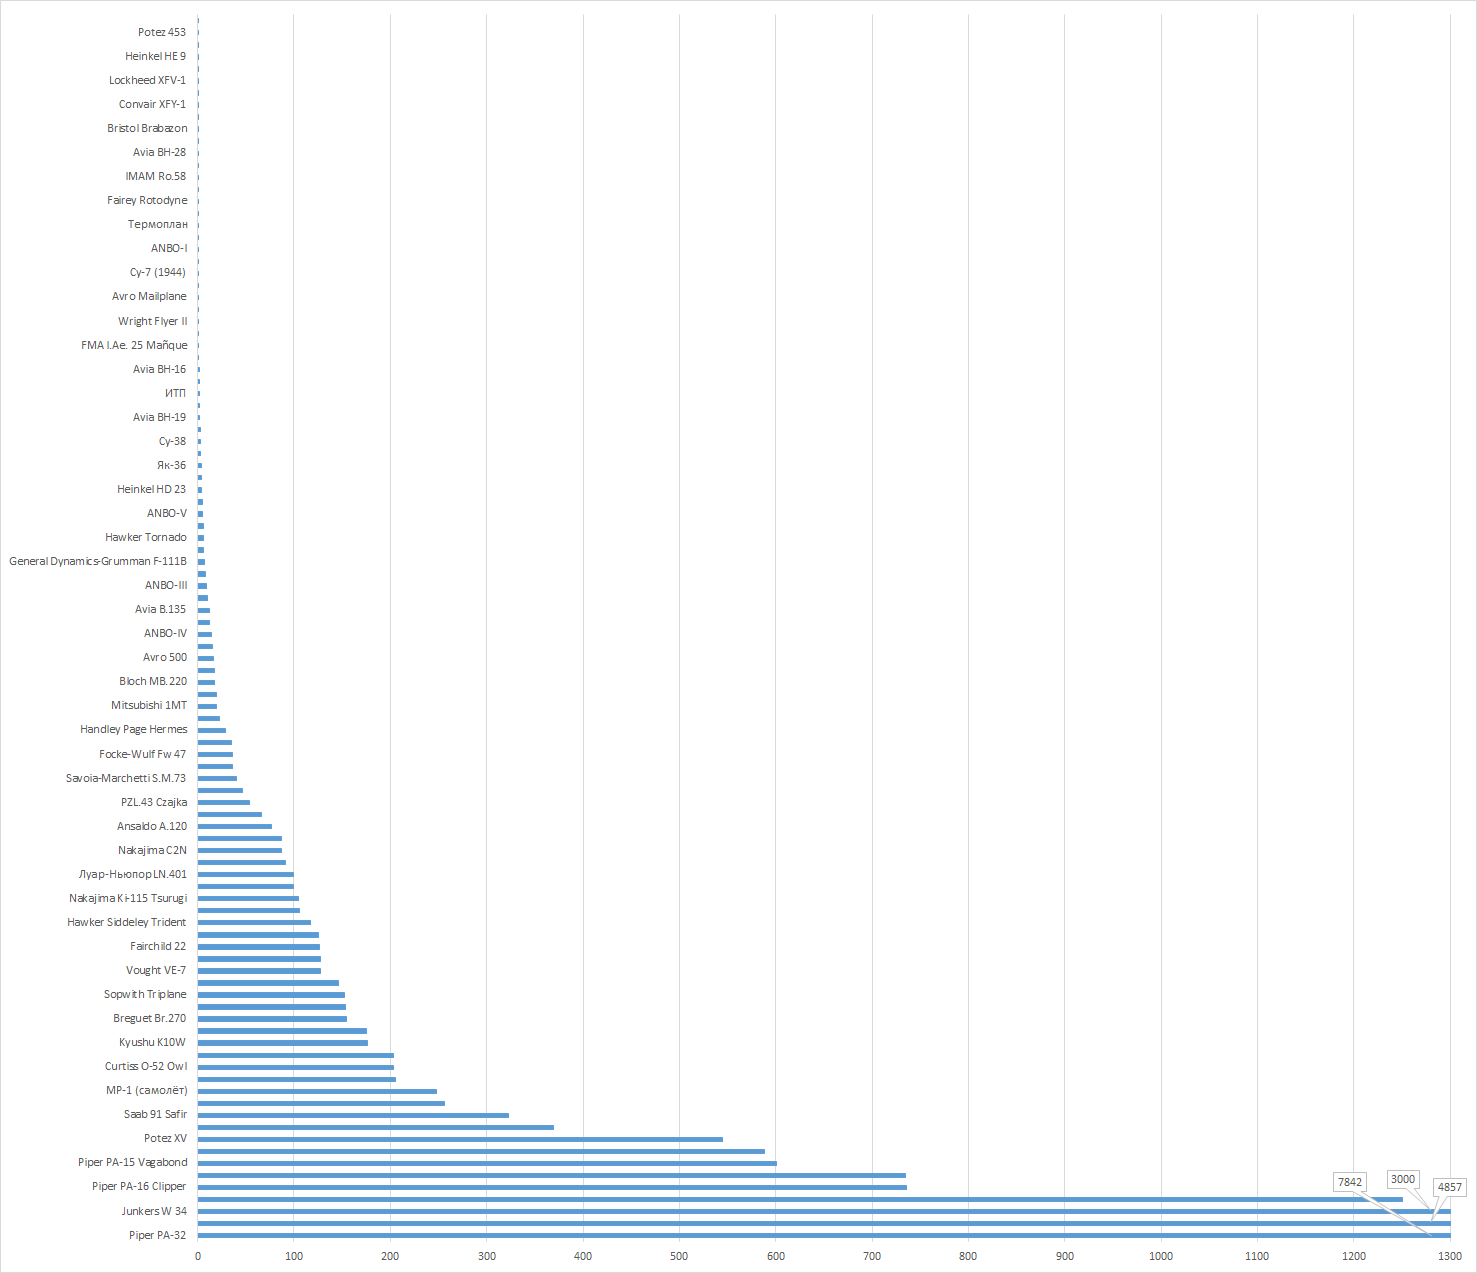
\includegraphics[width=\linewidth]{./chapter/aircraft/Number_of_aircraft_produced_ru.png}}%

%	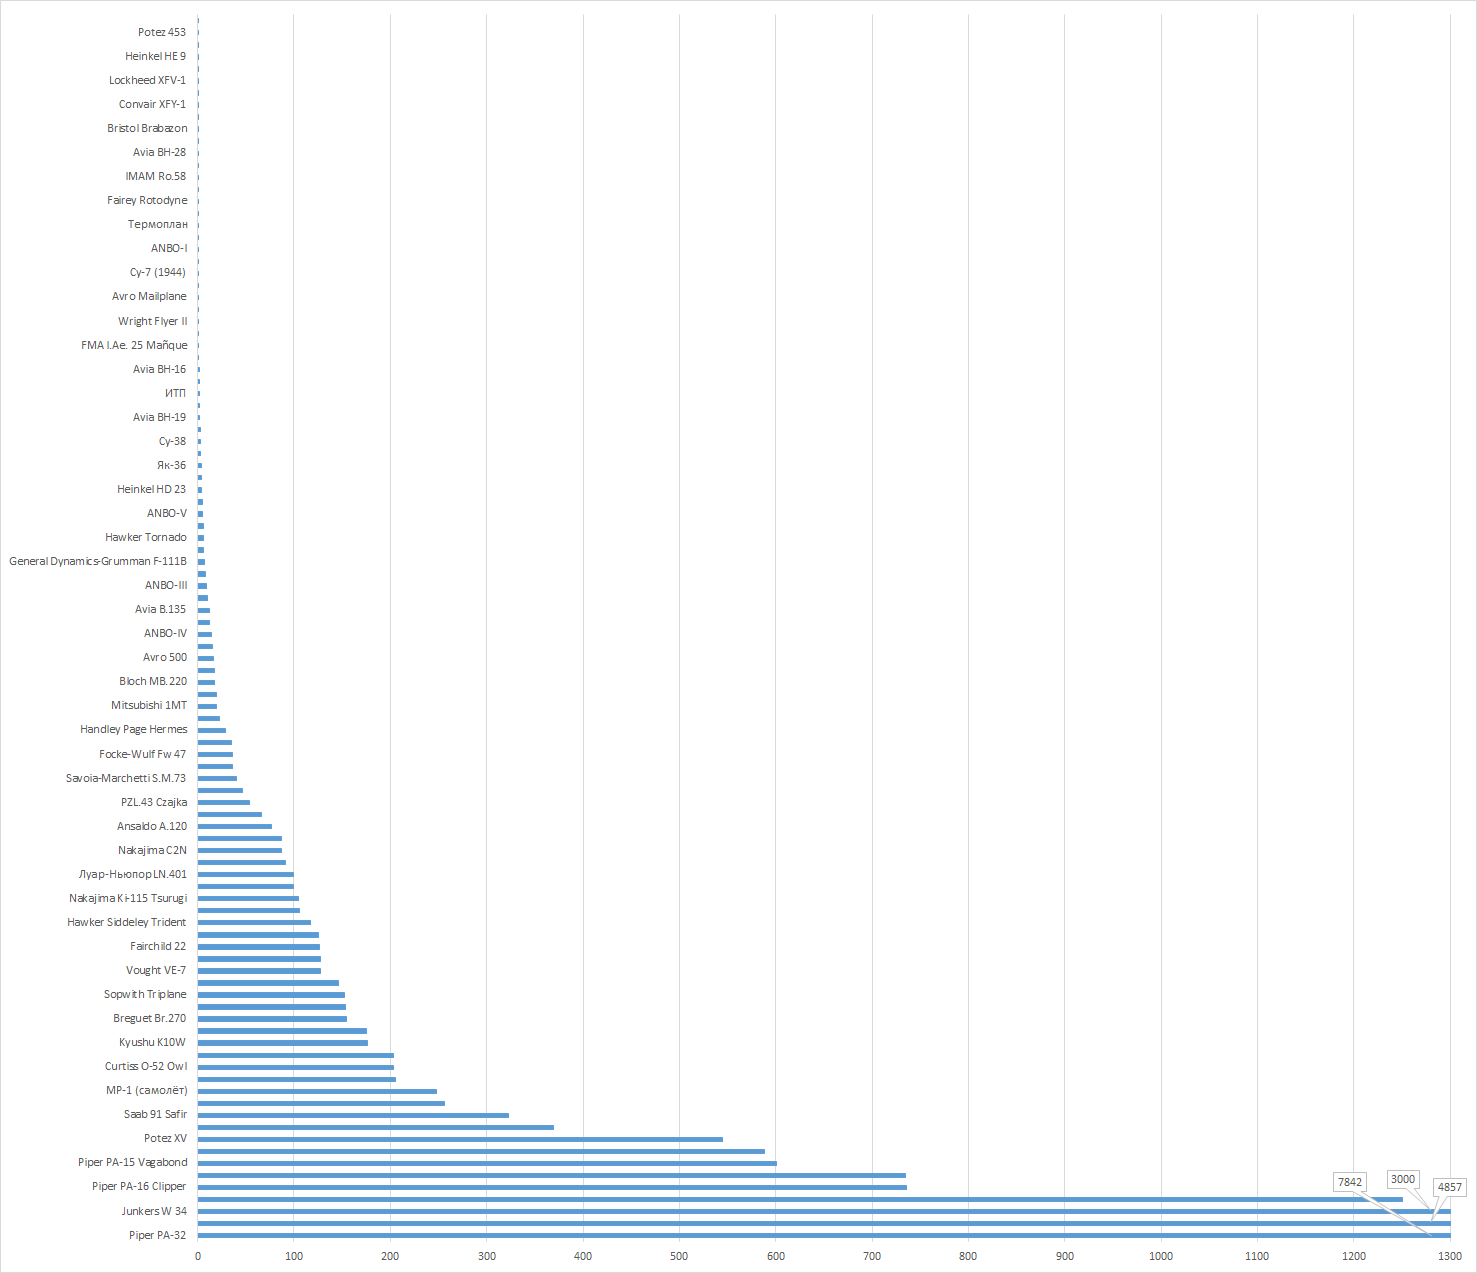
\includegraphics{./chapter/aircraft/Number_of_aircraft_produced_ru.png}%
	\caption{Количество выпущенных воздушных судов по моделям, 2020.}%
    \label{fig:Number_of_aircraft_produced_ru_2020}%
\end{figure*}

%По диаграмме видно, что больше всего было выпущено воздушных судов следующих моделей: Piper PA-32 (\num{7842} штук), Piper PA-24 Comanche (\num{4857}), Junkers W 34 (\num{3000}), Piper J-4 (\num{1251}).

Теперь попытаемся ответить на вопрос: <<Выполняется ли \href{https://clck.ru/JvaaU}{Закон Парето} относительно числа моделей самолётов>>?

Для того чтобы построить график необходимо выполнить следующие шаги:

\label{aircraft_question_2}
\marginnote{
Найдите соответствие между датой основания и компанией.
\\
\begin{tabular}{ l | l }
Компания & Дата основания \\ \hline
Миг & 01.01.1939 \\
Вымпел & 18.11.1949 \\
Туполев & 18.12.1939 \\
Сухой & 01.01.1922 \\
\end{tabular}
\\
См. ответ~\ref{answer:aircraft_company_foundation_date} на с.~\pageref{answer:aircraft_company_foundation_date}.
}

\begin{enumerate} 
  \item Подсчитать общее число самолётов по всем моделям. Для выполнения этой задачи был написан следующий скрипт:
  
  \begin{lstlisting}[ language=SPARQL, caption={\href{https://w.wiki/k36}{Общее число произведённых самолётов}\protect\footnotemark}, label=lst:lang3_2, ]
  SELECT (SUM(?count) as ?sum) WHERE {
    SELECT ?count WHERE {
      SERVICE wikibase:label { bd:serviceParam wikibase:language "ru". }
      ?item wdt:P31 wd:Q11436;
        wdt:P1092 ?count.
    }
  }
  \end{lstlisting}
  \footnotetext{Общее число выпущенных самолётов на 2020 год состовляет \num{33177}. Ссылка на SPARQL-запрос: \href{https://w.wiki/k36}{https://w.wiki/k36}}
  
  %В результате выполнения запроса ~\ref{lst:lang3_2} мы получили общее число выпущенных самолётов на 2020 год = \num{33177}.
  
  \item По оси Х - число рассматриваемых моделей самолётов (то есть 1 - количество выпущенных самолётов 1-ой модели, 2 - сумма выпущенных самолётов 1-ой и 2-ой модели и т.д.). По оси Y будем откладывать процентное соотношение количества выпущенных моделей самолётов к общему числу выпущенных самолётов за всё время. Также по оси Х откладываем вторую шкалу от 0 до 100%, чтобы легче было определить параметры для закона Парето.
\end{enumerate}

\begin{figure*}[h]

    \setlength{\fboxsep}{0pt}%
    \setlength{\fboxrule}{1pt}%
    \fcolorbox{gray}{gray}{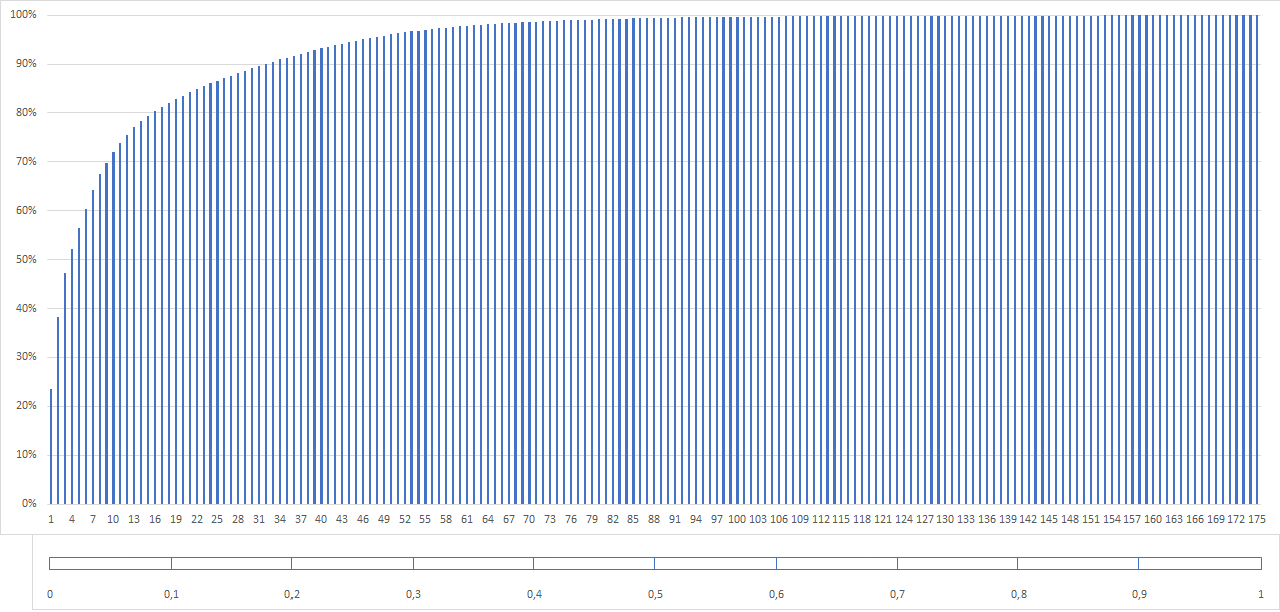
\includegraphics[width=\linewidth]{./chapter/aircraft/Pareto_principle_diargam.png}}%

%	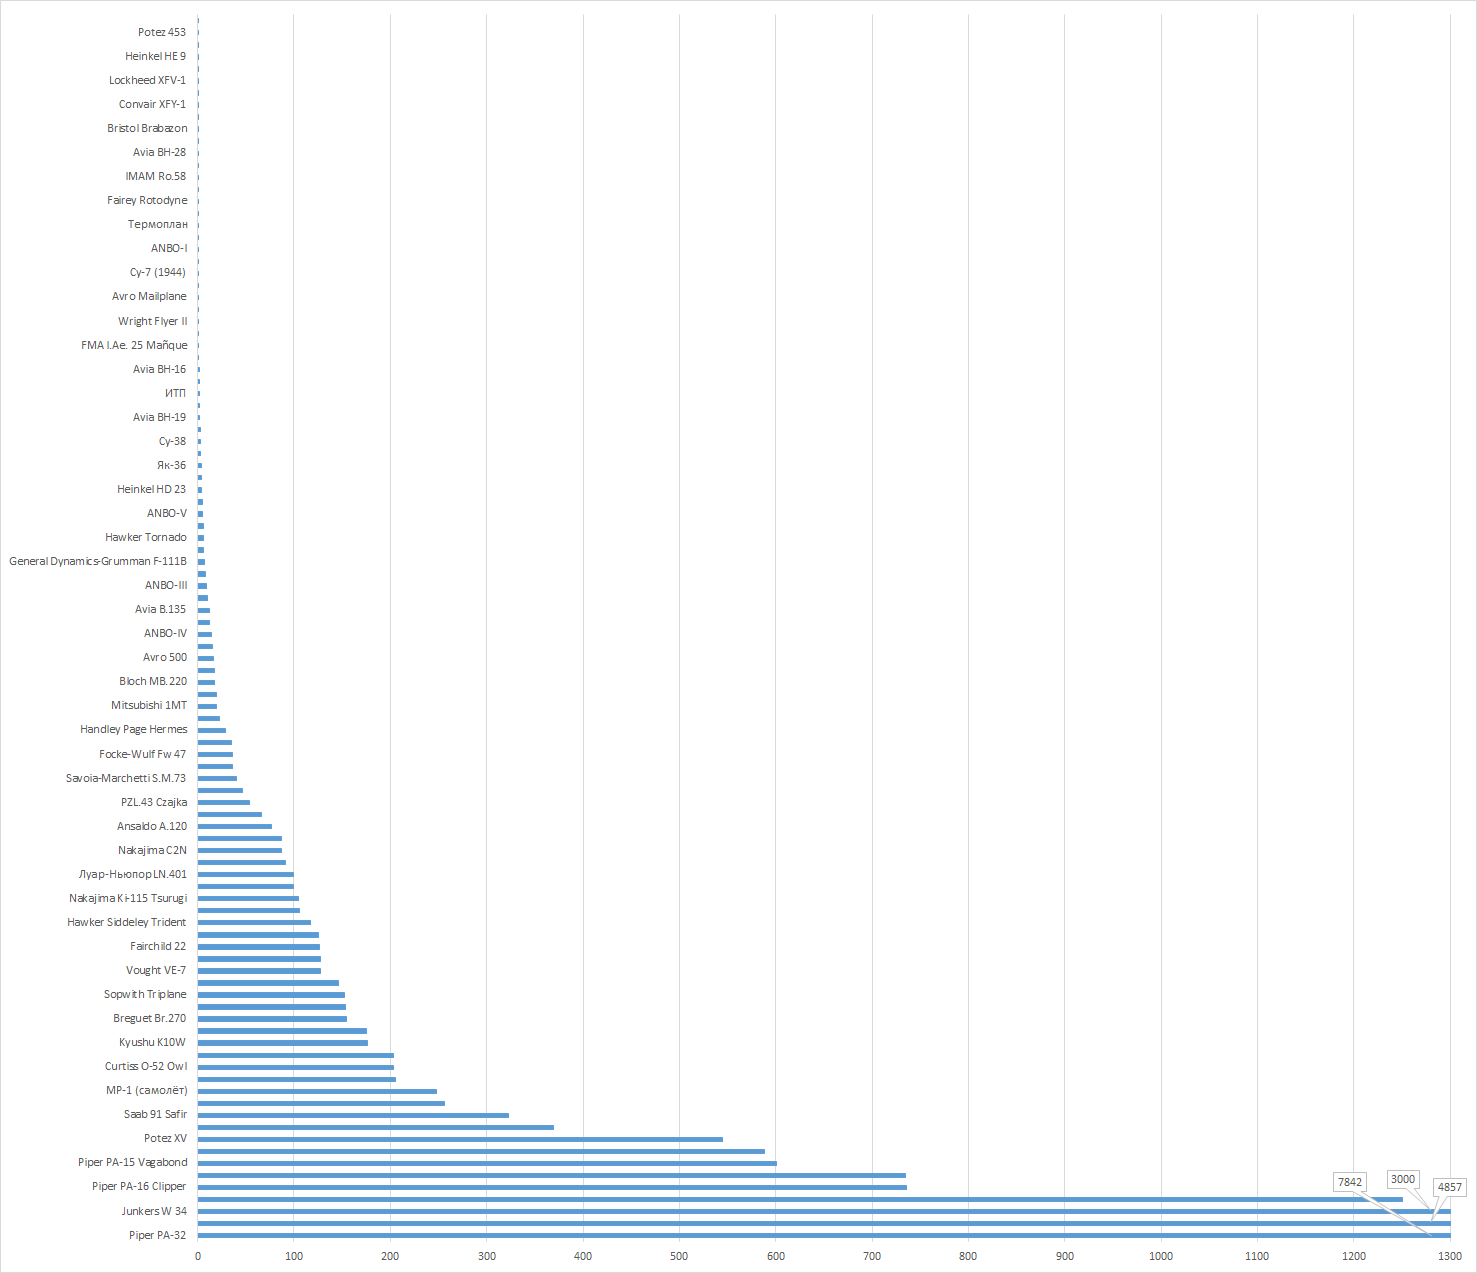
\includegraphics{./chapter/aircraft/Number_of_aircraft_produced_ru.png}%
	\caption{Распределение числа выпущенных моделей самолётов, 2020.}%
    \label{fig:Pareto_principle_diargam}%
\end{figure*}

По графику видно, что 80\% всех выпущенных самолётов приходится на 16 различных моделей самолётов, что составляет 9,2\% от общего числа моделей. Закон Парето утверждает, что: «20\% усилий дают 80\% результата, а остальные 80\% усилий — лишь 20\% результата». Можно сделать вывод, что выполняется более сильный закон, чем принцип Парето относительно числа моделей самолётов.


\section{Страны происхождения производителей воздушных судов}

Построим список с соотношением количества производителей воздушных судов по странам. Для выполнения запроса используем группировку по странам (GROUP BY) и при помощи функции <<Count>> для каждой страны подсчитаем количество производств.

\label{aircraft_question_3}
\marginnote{
Найдите соответствие между расположением штаб-квартирой компании и компанией.
\\
\begin{tabular}{ l | l }
Компания & Штаб-квартира \\ \hline
Камов & Улан-Удэ \\
Авиадвигатель & Пермь \\
Улан-Удэнский & Москва \\
авиационный завод \\
Сухой & Люберцы \\
\end{tabular}
\\
См. ответ~\ref{answer:aircraft_company_headquarters} на с.~\pageref{answer:aircraft_company_headquarters}.
}

\begin{lstlisting}[ language=SPARQL, caption={\href{https://w.wiki/kYJ}{Список соотношения количества производителей воздушных судов по странам}\protect\footnotemark}, label=lst:lang4, ]
# Count manufacture having property country
# group by country
SELECT ?countryLabel (count(?item) as ?count)
WHERE
{
    ?item wdt:P31 wd:Q936518.   # instance of manufacture
    ?item wdt:P17 ?country.     # show country
    SERVICE wikibase:label { bd:serviceParam wikibase:language "ru" }
}
GROUP BY ?country ?countryLabel # group by country
\end{lstlisting}
\footnotetext{Получено 39 записей (страна и количество производств воздушных судов) в 2017 году, 46 записей в 2020 году. Ссылка на SPARQL-запрос: \href{https://w.wiki/kYJ}{https://w.wiki/kYJ}}

%В результатом запроса ~\ref{lst:lang4} мы получили список состоящий из 39 записей (на 2017 год): страна и количество производств воздушных судов. К 2020 году число записей в руском сегменте Викиданных возросло до 46 записей.

Получив общий список количества производств по странам, мы можем для наглядности построить пузырьковую диаграмму. Для её построения выполняем следующий запрос:

\begin{lstlisting}[ language=SPARQL, caption={\href{https://w.wiki/kYL}{Пузырьковая диаграмма}}, label=lst:lang5, ]
#defaultView:BubbleChart
SELECT ?countryLabel (count(?item) as ?count)
WHERE
{
    ?item wdt:P31 wd:Q936518.
  	?item wdt:P17 ?country.
    SERVICE wikibase:label { bd:serviceParam wikibase:language "ru" }
}
GROUP BY ?country ?countryLabel
\end{lstlisting}
\footnotetext{Ссылка на SPARQL-запрос: \href{https://w.wiki/kYL}{https://w.wiki/kYL}}

В результате выполнения запроса ~\ref{lst:lang5} будет построена пузырьковая диаграмма, в которой круги означают страны, а их размеры соответствуют количеству авиапроизводителей в данной стране. Такая диаграмма помогает более наглядно увидеть разницу между объектами.
 
\begin{figure}[h!]
\centering
	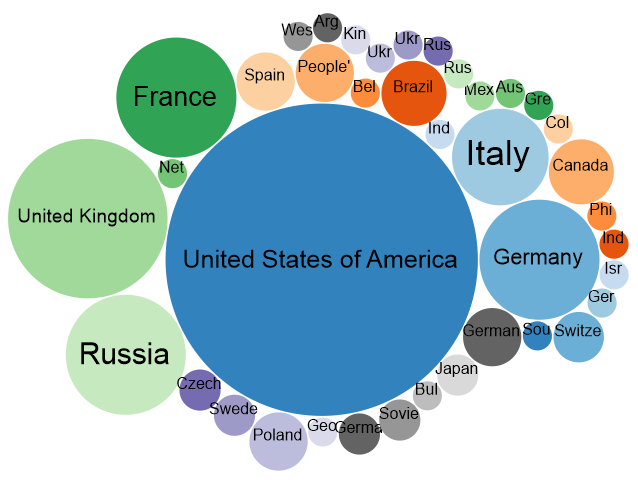
\includegraphics[width=0.7\textwidth]{./chapter/aircraft/Manufacture-with-country_2017.png}
	\caption{Соотношение количества производителей воздушных судов по странам 2017 год.}
	\label{fig:Manufacture_with_country_2017}
\end{figure}

Как видно из ответа на запрос ~\ref{lst:lang5} на (рис. ~\ref{fig:Manufacture_with_country_2017}), страны происхождения указаны у производителей воздушных судов куда хуже, чем могли бы быть, и предоставляют мало информации. Больше всего производителей указано у США (115), Великобритании (30), Германии (17), России (17) на май 2017.

\begin{figure}[h!]
\centering
	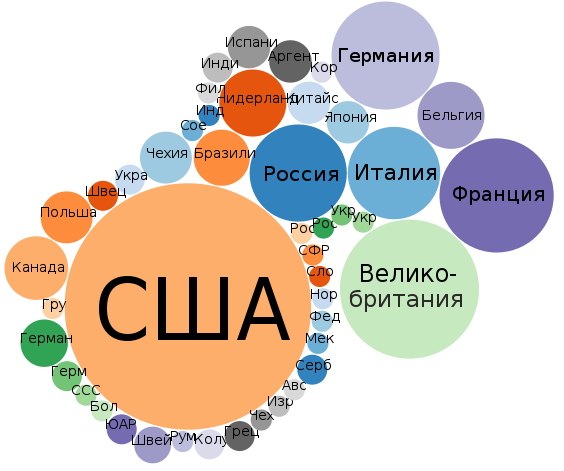
\includegraphics[width=0.7\textwidth]{./chapter/aircraft/Manufacture-with-country_2020.png}
	\caption{Соотношение количества производителей воздушных судов по странам 2020 год.}
	\label{fig:Manufacture_with_country_2020}
\end{figure}

\label{aircraft_question_4}
\marginnote{
Как называется воздушное судно, поддерживаемое в полете за счёт огромного баллона с горючим смертельно опасным газом, прямо над головой пассажиров?
\\
См. ответ~\ref{answer:aircraft_question_airship} на с.~\pageref{answer:aircraft_question_airship}.
}

Сравнивая 2 пузырьковые диаграммы за 2017 (рис. ~\ref{fig:Manufacture_with_country_2017}) и 2020 (рис. ~\ref{fig:Manufacture_with_country_2020}) года, можно сделать вывод, что основными производителями воздушных судов являются: США (135), Великобритания (43), Франция (29), Германия (26), Россия (21). Лидером по прежнему является США, а вот Франция за 3 года сумела опередить Германия, заняв 3-е место. Но в целом соотношение по производству воздушных судов между различными странами остаётся на прежнем уровне.

\section{Полнота Викиданных}

\label{aircraft_question_5}
\marginnote{
Какое воздушное судно изображено на рис. \ref{fig:airship_question_aircraft}?
}


\begin{marginfigure}[0.0cm]
{
\setlength{\fboxsep}{0pt}%
\setlength{\fboxrule}{1pt}%
\fcolorbox{gray}{gray}{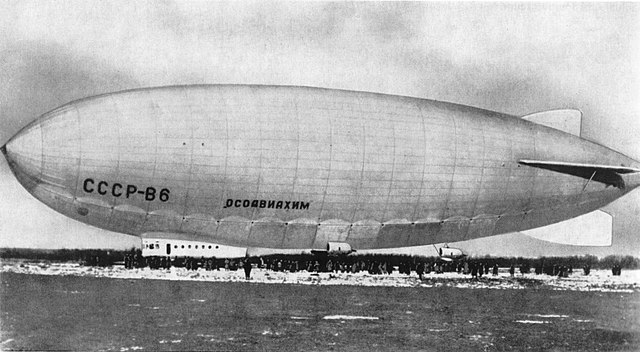
\includegraphics[width=\linewidth]{./chapter/aircraft/foto_of_airship.jpg}}%
}
  \caption{Воздушное судно}%
  \label{fig:airship_question_aircraft}%
\end{marginfigure}

\marginnote{
См. ответ~\ref{answer:aircraft_question_airship_2} на с.~\pageref{answer:aircraft_question_airship_2}.
}

Согласно сайту \href{https://www.aviationfanatic.com/}{aviationfanatic.com} существует около \num{1700} производителей воздушных судов, но SPARQL-запрос ~\ref{lst:lang2} вернул всего 300 записей. Из этого можно сделать вывод о неполноте Викиданных. Скорее всего, оставшиеся полторы тысячи производителей сделали слишком мало самолетов или не сделали их вовсе, поэтому из-за недостатка информации они не были включены в Викиданные.

В категории Авиастроительные компании России указано наличие в России 58 авиастроительных компании, но в то же время на сайте aviationfanatic.com указано наличие 61 завода, например такие компании как \href{https://clck.ru/RxFCs}{Иркут}, \href{https://clck.ru/QR6qZ}{МиГ}, \href{https://clck.ru/RxFG3}{Туполев}.

%\section{Степень заполненности Викиданных}

%Для заполнения были выбраны поля label и description у объектов, перечисленных в категории <<Авиастроительные компании России>>. Так как объектов там много, было решено автоматизировать заполнение, для чего была написана соответствующая программа. Для начала был создан JSON-файл с объектами из категории и пустыми полями для заполнения:

%\begin{lstlisting}[ language=SPARQL, label=lst:lang6, ]
%{
%  "121 авиационный ремонтный завод": {
%    "description": "",
%    "descriptionen": "",
%    "nameen": "",
%    "qid": "Q4028573"
%    },
%  ...
%}
%\end{lstlisting}

%В первой части программы записывались уже существующие значения полей из Викиданных в JSON-файл. После чего было необходимо заполнить оставшиеся пустыми поля, то есть поля, не заполненые в Викиданных. В итоге JSON-файл выглядел примерно так:

%\begin{lstlisting}[ language=SPARQL, label=lst:lang7, ]
%{
%  "121 авиационный ремонтный завод": {
%    "description": "авиаремонтное предприятие, расположенное посёлке Старый Городок",
%    "descriptionen": "aircraft repair facility, located in the village Stary Gorodok",
%    "nameen": "121 aircraft repair plant",
%    "qid": "Q4028573"
%  },
%  ...
%}
%\end{lstlisting}

%Во второй части программы записывались данные из JSON-файла в Викиданные.

%С помощью этой программы удалось упростить работу с Викиданными, так как не приходилось самостоятельно заходить на страницы объектов и вносить изменения, если существующие данные не удовлетворяют ожиданиям, то есть поле в Викиданных отличается от локального.

\section{Упражнения}
\begin{enumerate}
\item Найти самолет с максимальным радиусом полета.
\item Отметить на политической карте главные офисы компаний авиапроизводителей.
\item Найти производителя с максимальным числом изготовленных самолетов, используя свойство manufacturer у воздушных судов.
\end{enumerate}
